

\tikzset{every picture/.style={line width=0.75pt}} %set default line width to 0.75pt        

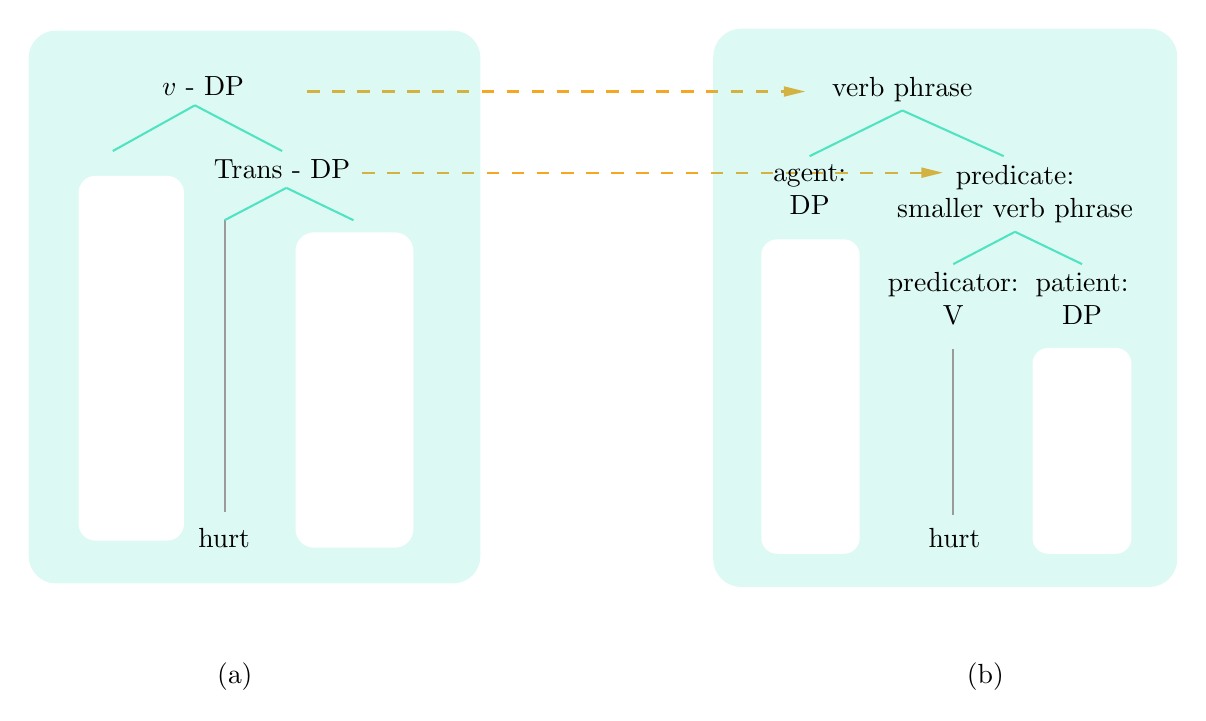
\begin{tikzpicture}[x=0.75pt,y=0.75pt,yscale=-0.85,xscale=0.85]
%uncomment if require: \path (0,408); %set diagram left start at 0, and has height of 408

%Straight Lines [id:da2665478368972569] 
\draw [color={rgb, 255:red, 245; green, 166; blue, 35 }  ,draw opacity=1 ] [dash pattern={on 4.5pt off 4.5pt}]  (264,61) -- (544,61) ;
\draw [shift={(546,61)}, rotate = 180] [fill={rgb, 255:red, 245; green, 166; blue, 35 }  ,fill opacity=1 ][line width=0.08]  [draw opacity=0] (12,-3) -- (0,0) -- (12,3) -- cycle    ;
%Straight Lines [id:da6278442099042232] 
\draw [color={rgb, 255:red, 245; green, 166; blue, 35 }  ,draw opacity=1 ] [dash pattern={on 4.5pt off 4.5pt}]  (295,107) -- (622,107) ;
\draw [shift={(624,107)}, rotate = 180] [fill={rgb, 255:red, 245; green, 166; blue, 35 }  ,fill opacity=1 ][line width=0.08]  [draw opacity=0] (12,-3) -- (0,0) -- (12,3) -- cycle    ;
%Rounded Rect [id:dp9005470977487176] 
\draw  [draw opacity=0][fill={rgb, 255:red, 80; green, 227; blue, 194 }  ,fill opacity=0.2 ] (494,41.22) .. controls (494,32.48) and (501.08,25.4) .. (509.82,25.4) -- (741.18,25.4) .. controls (749.92,25.4) and (757,32.48) .. (757,41.22) -- (757,325.99) .. controls (757,334.73) and (749.92,341.81) .. (741.18,341.81) -- (509.82,341.81) .. controls (501.08,341.81) and (494,334.73) .. (494,325.99) -- cycle ;
%Straight Lines [id:da3555404365615693] 
\draw [color={rgb, 255:red, 155; green, 155; blue, 155 }  ,draw opacity=1 ]   (630.05,206.81) -- (630.05,301) ;
%Straight Lines [id:da5116688308518689] 
\draw [color={rgb, 255:red, 80; green, 227; blue, 194 }  ,draw opacity=1 ]   (703.05,158.83) -- (665.05,140.5) ;
%Straight Lines [id:da7532901881200198] 
\draw [color={rgb, 255:red, 80; green, 227; blue, 194 }  ,draw opacity=1 ]   (665.05,140.5) -- (630.05,158.83) ;
%Straight Lines [id:da3708728686228633] 
\draw [color={rgb, 255:red, 80; green, 227; blue, 194 }  ,draw opacity=1 ]   (658.65,97.63) -- (601.2,71.73) ;
%Straight Lines [id:da18650265857430104] 
\draw [color={rgb, 255:red, 80; green, 227; blue, 194 }  ,draw opacity=1 ]   (601.2,71.73) -- (548.65,97.63) ;
%Rounded Rect [id:dp9951745940140804] 
\draw  [draw opacity=0][fill={rgb, 255:red, 255; green, 255; blue, 255 }  ,fill opacity=1 ] (675,215.16) .. controls (675,210.29) and (678.95,206.33) .. (683.83,206.33) -- (722.17,206.33) .. controls (727.05,206.33) and (731,210.29) .. (731,215.16) -- (731,314.17) .. controls (731,319.05) and (727.05,323) .. (722.17,323) -- (683.83,323) .. controls (678.95,323) and (675,319.05) .. (675,314.17) -- cycle ;
%Rounded Rect [id:dp4970986462373306] 
\draw  [draw opacity=0][fill={rgb, 255:red, 255; green, 255; blue, 255 }  ,fill opacity=1 ] (521.24,153.76) .. controls (521.24,148.82) and (525.25,144.81) .. (530.19,144.81) -- (568.05,144.81) .. controls (572.99,144.81) and (577,148.82) .. (577,153.76) -- (577,314.05) .. controls (577,318.99) and (572.99,323) .. (568.05,323) -- (530.19,323) .. controls (525.25,323) and (521.24,318.99) .. (521.24,314.05) -- cycle ;
%Rounded Rect [id:dp4071663798075751] 
\draw  [draw opacity=0][fill={rgb, 255:red, 80; green, 227; blue, 194 }  ,fill opacity=0.2 ] (106,41.89) .. controls (106,33.39) and (112.89,26.5) .. (121.4,26.5) -- (346.6,26.5) .. controls (355.11,26.5) and (362,33.39) .. (362,41.89) -- (362,324.41) .. controls (362,332.92) and (355.11,339.81) .. (346.6,339.81) -- (121.4,339.81) .. controls (112.89,339.81) and (106,332.92) .. (106,324.41) -- cycle ;
%Straight Lines [id:da5088138181155522] 
\draw [color={rgb, 255:red, 155; green, 155; blue, 155 }  ,draw opacity=1 ]   (217.05,133.93) -- (217.05,299.1) ;
%Straight Lines [id:da998446713157706] 
\draw [color={rgb, 255:red, 80; green, 227; blue, 194 }  ,draw opacity=1 ]   (290.05,133.93) -- (252.05,115.6) ;
%Straight Lines [id:da5752866187220778] 
\draw [color={rgb, 255:red, 80; green, 227; blue, 194 }  ,draw opacity=1 ]   (252.05,115.6) -- (217.05,133.93) ;
%Straight Lines [id:da6021628337779128] 
\draw [color={rgb, 255:red, 80; green, 227; blue, 194 }  ,draw opacity=1 ]   (249.65,94.73) -- (200.2,68.83) ;
%Straight Lines [id:da8361003247119008] 
\draw [color={rgb, 255:red, 80; green, 227; blue, 194 }  ,draw opacity=1 ]   (200.2,68.83) -- (153.65,94.73) ;
%Rounded Rect [id:dp3858870486231194] 
\draw  [draw opacity=0][fill={rgb, 255:red, 255; green, 255; blue, 255 }  ,fill opacity=1 ] (257.24,151.34) .. controls (257.24,145.52) and (261.96,140.81) .. (267.77,140.81) -- (313.48,140.81) .. controls (319.29,140.81) and (324,145.52) .. (324,151.34) -- (324,309.05) .. controls (324,314.86) and (319.29,319.57) .. (313.48,319.57) -- (267.77,319.57) .. controls (261.96,319.57) and (257.24,314.86) .. (257.24,309.05) -- cycle ;
%Rounded Rect [id:dp2951833006567197] 
\draw  [draw opacity=0][fill={rgb, 255:red, 255; green, 255; blue, 255 }  ,fill opacity=1 ] (134.24,118.4) .. controls (134.24,113.11) and (138.54,108.81) .. (143.84,108.81) -- (184.41,108.81) .. controls (189.71,108.81) and (194,113.11) .. (194,118.4) -- (194,305.98) .. controls (194,311.28) and (189.71,315.57) .. (184.41,315.57) -- (143.84,315.57) .. controls (138.54,315.57) and (134.24,311.28) .. (134.24,305.98) -- cycle ;

% Text Node
\draw (630.76,321) node [anchor=south] [inner sep=0.75pt]   [align=left] {hurt};
% Text Node
\draw (665.05,137.5) node [anchor=south] [inner sep=0.75pt]   [align=left] {\begin{minipage}[lt]{89.53pt}\setlength\topsep{0pt}
\begin{center}
predicate:\\smaller verb phrase
\end{center}

\end{minipage}};
% Text Node
\draw (601.2,68.73) node [anchor=south] [inner sep=0.75pt]   [align=left] {verb phrase};
% Text Node
\draw (548.65,100.63) node [anchor=north] [inner sep=0.75pt]   [align=left] {\begin{minipage}[lt]{29.61pt}\setlength\topsep{0pt}
\begin{center}
agent:\\DP
\end{center}

\end{minipage}};
% Text Node
\draw (630.05,161.83) node [anchor=north] [inner sep=0.75pt]   [align=left] {\begin{minipage}[lt]{50.89pt}\setlength\topsep{0pt}
\begin{center}
predicator:\\V
\end{center}

\end{minipage}};
% Text Node
\draw (703.05,161.83) node [anchor=north] [inner sep=0.75pt]   [align=left] {\begin{minipage}[lt]{36.95pt}\setlength\topsep{0pt}
\begin{center}
patient:\\DP
\end{center}

\end{minipage}};
% Text Node
\draw (216.76,321.1) node [anchor=south] [inner sep=0.75pt]   [align=left] {hurt};
% Text Node
\draw (249.65,97.73) node [anchor=north] [inner sep=0.75pt]   [align=left] {Trans - DP};
% Text Node
\draw (179.8,50.81) node [anchor=north west][inner sep=0.75pt]   [align=left] {$\displaystyle v$ - DP};
% Text Node
\draw (211,383) node [anchor=north west][inner sep=0.75pt]   [align=left] {(a)};
% Text Node
\draw (636,383) node [anchor=north west][inner sep=0.75pt]   [align=left] {(b)};


\end{tikzpicture}
